% implementation structures O(1), Vertex, Triangle, Observables

% Store the geometry
% Naïve solution: use slice structure to store a sequence of up-down
% Performing moves meaning moving triangles, meaning O(N) complexity
% Solution: store list with connectivities
% Distances are of intrest so natural to look at connectivity of vertices
% Computationally simplier is to look at connectivity of triangles
% Finally: store an ordered list where every element represents a triangle, which stores the triangle indices it is connected to, and it's type (up-down)
% In this way both moves can be done in O(1), the 4-4 move without rejection and the 2-2 flip with rejection rate of approximately 50%

% To be able to analyse the behaviour of the model, meaningful observables need to be found
% These observables cannot depend on the labels, and have no 'positional' information, as the system is fully periodic
% Interesting to look at the behaviour of the spatial size of the universe: here simply counting the number of space-like links on the boundaries of the timeslices; this already gets rid of the spatial dependence.
% To get rid of the time dependence we can perform an average (this is trivially L as we keep N constant), look at the standard deviation, look at the autocorrelation of spatial size over time (using periodic boundaries, to be able to do so T need to be sufficiently large).

% To get the length profile out of the adjacency data we 'walk' through the triangulation along slices first (recording the amount of up-triangles) until going around fully; then advance up via a down triangle and repeat; until the original slice is again reached.
% For visualisation of the triangulation we do something similar but in stead of counting the number of up-triangles, we label the vertices and record to which triangle they belong; in the end yielding a list of triangles each with three labels to vertices
% Then we choose an embedding, one that obeys the slice behaviour, meaning the coordinates of the vertices are chosen; from this the triangulation can be visualized. This embedding may also be 2D 


\begin{frame}
    \frametitle{Observables}

    
    \begin{itemize}
        \item Difficult to find meaningful observables
        \item Cannot depend on labeling $\rightarrow$ average over geometry
        \item ...
    \end{itemize}
    \begin{figure}
       \centering
       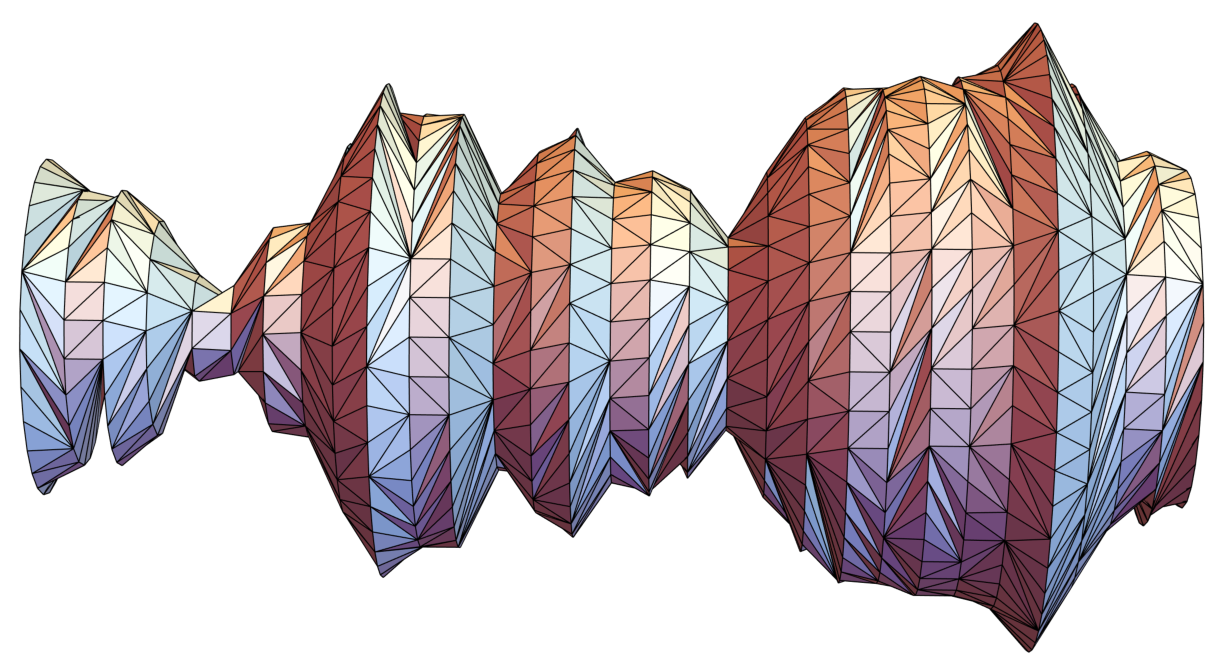
\includegraphics[width=0.6\linewidth]{img/triangulation.pdf}    
    \end{figure}

\end{frame}